
\thispagestyle{fancy}


\section{Rekombinationsmechanismen}

\begin{figure}[htb]
    \centering
    \begin{minipage}[t]{0.49\linewidth}
        \centering
        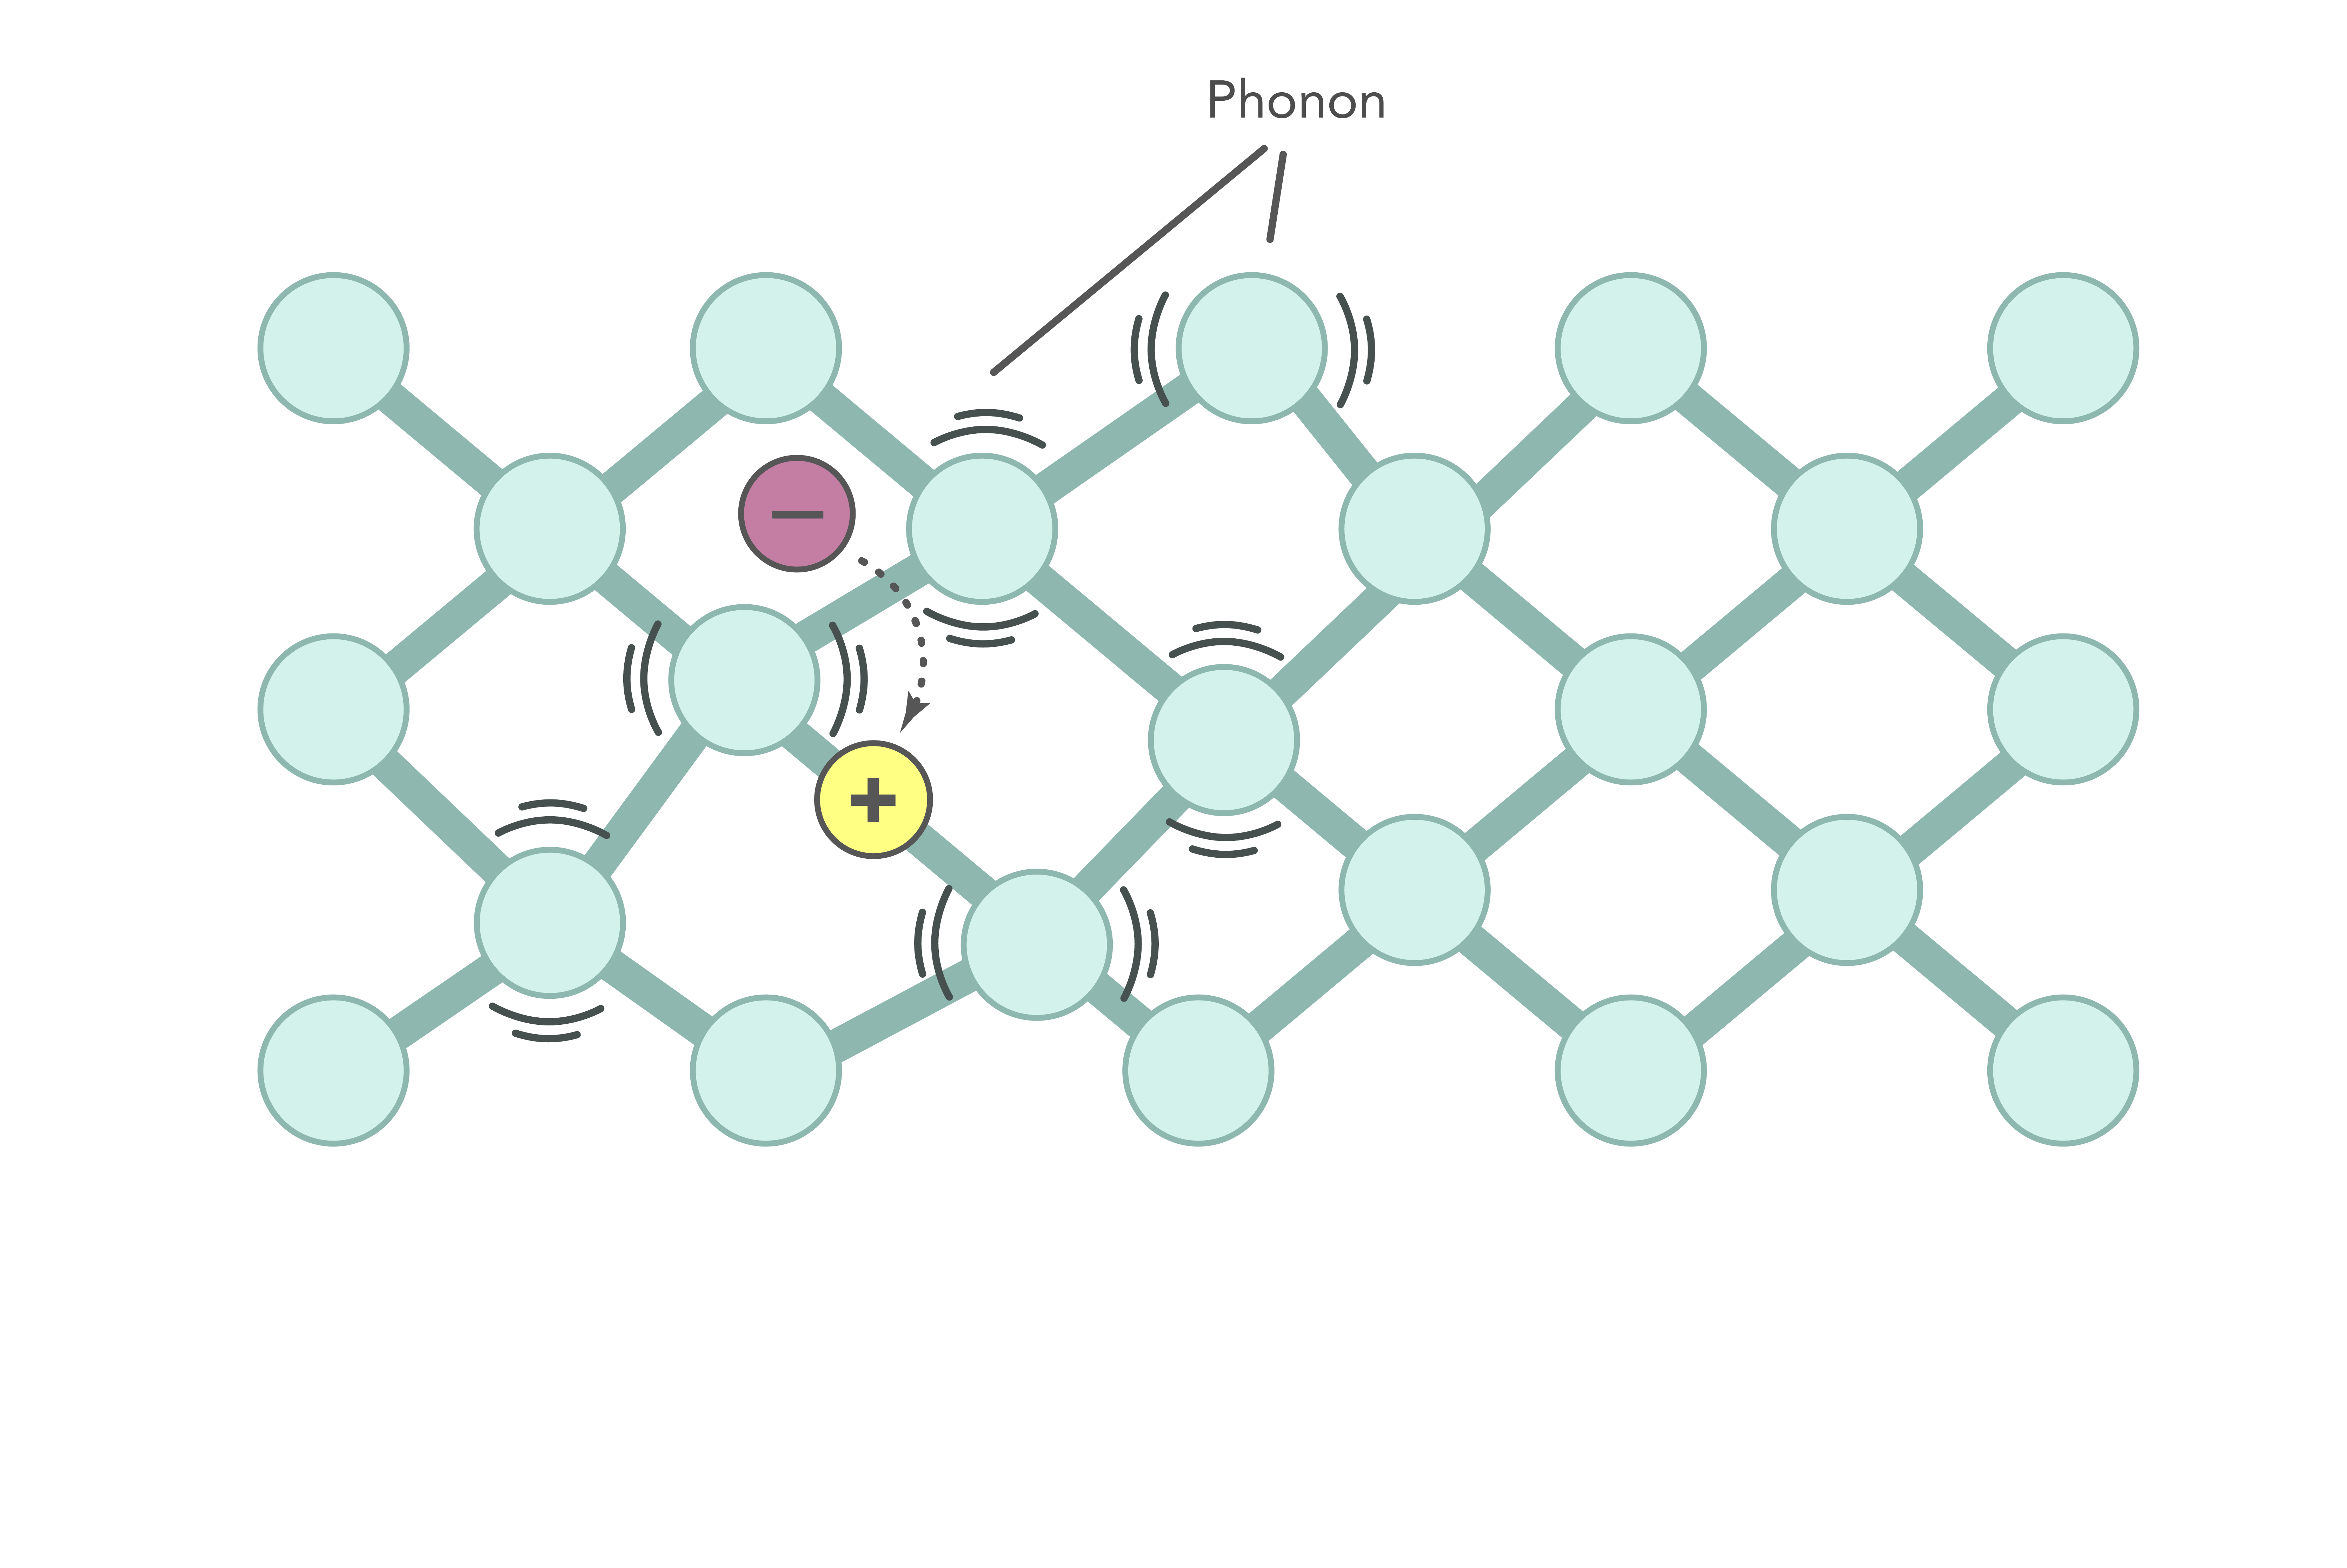
\includegraphics[width=\linewidth]{Bilder/nonradRekomb.png}
        \caption{Rekombination von Elektron und Loch unter Teilnahme eines Phonons.}
    \end{minipage}% <- sonst wird hier ein Leerzeichen eingefügt
    \hfill
    \begin{minipage}[t]{0.49\linewidth}
        \centering
        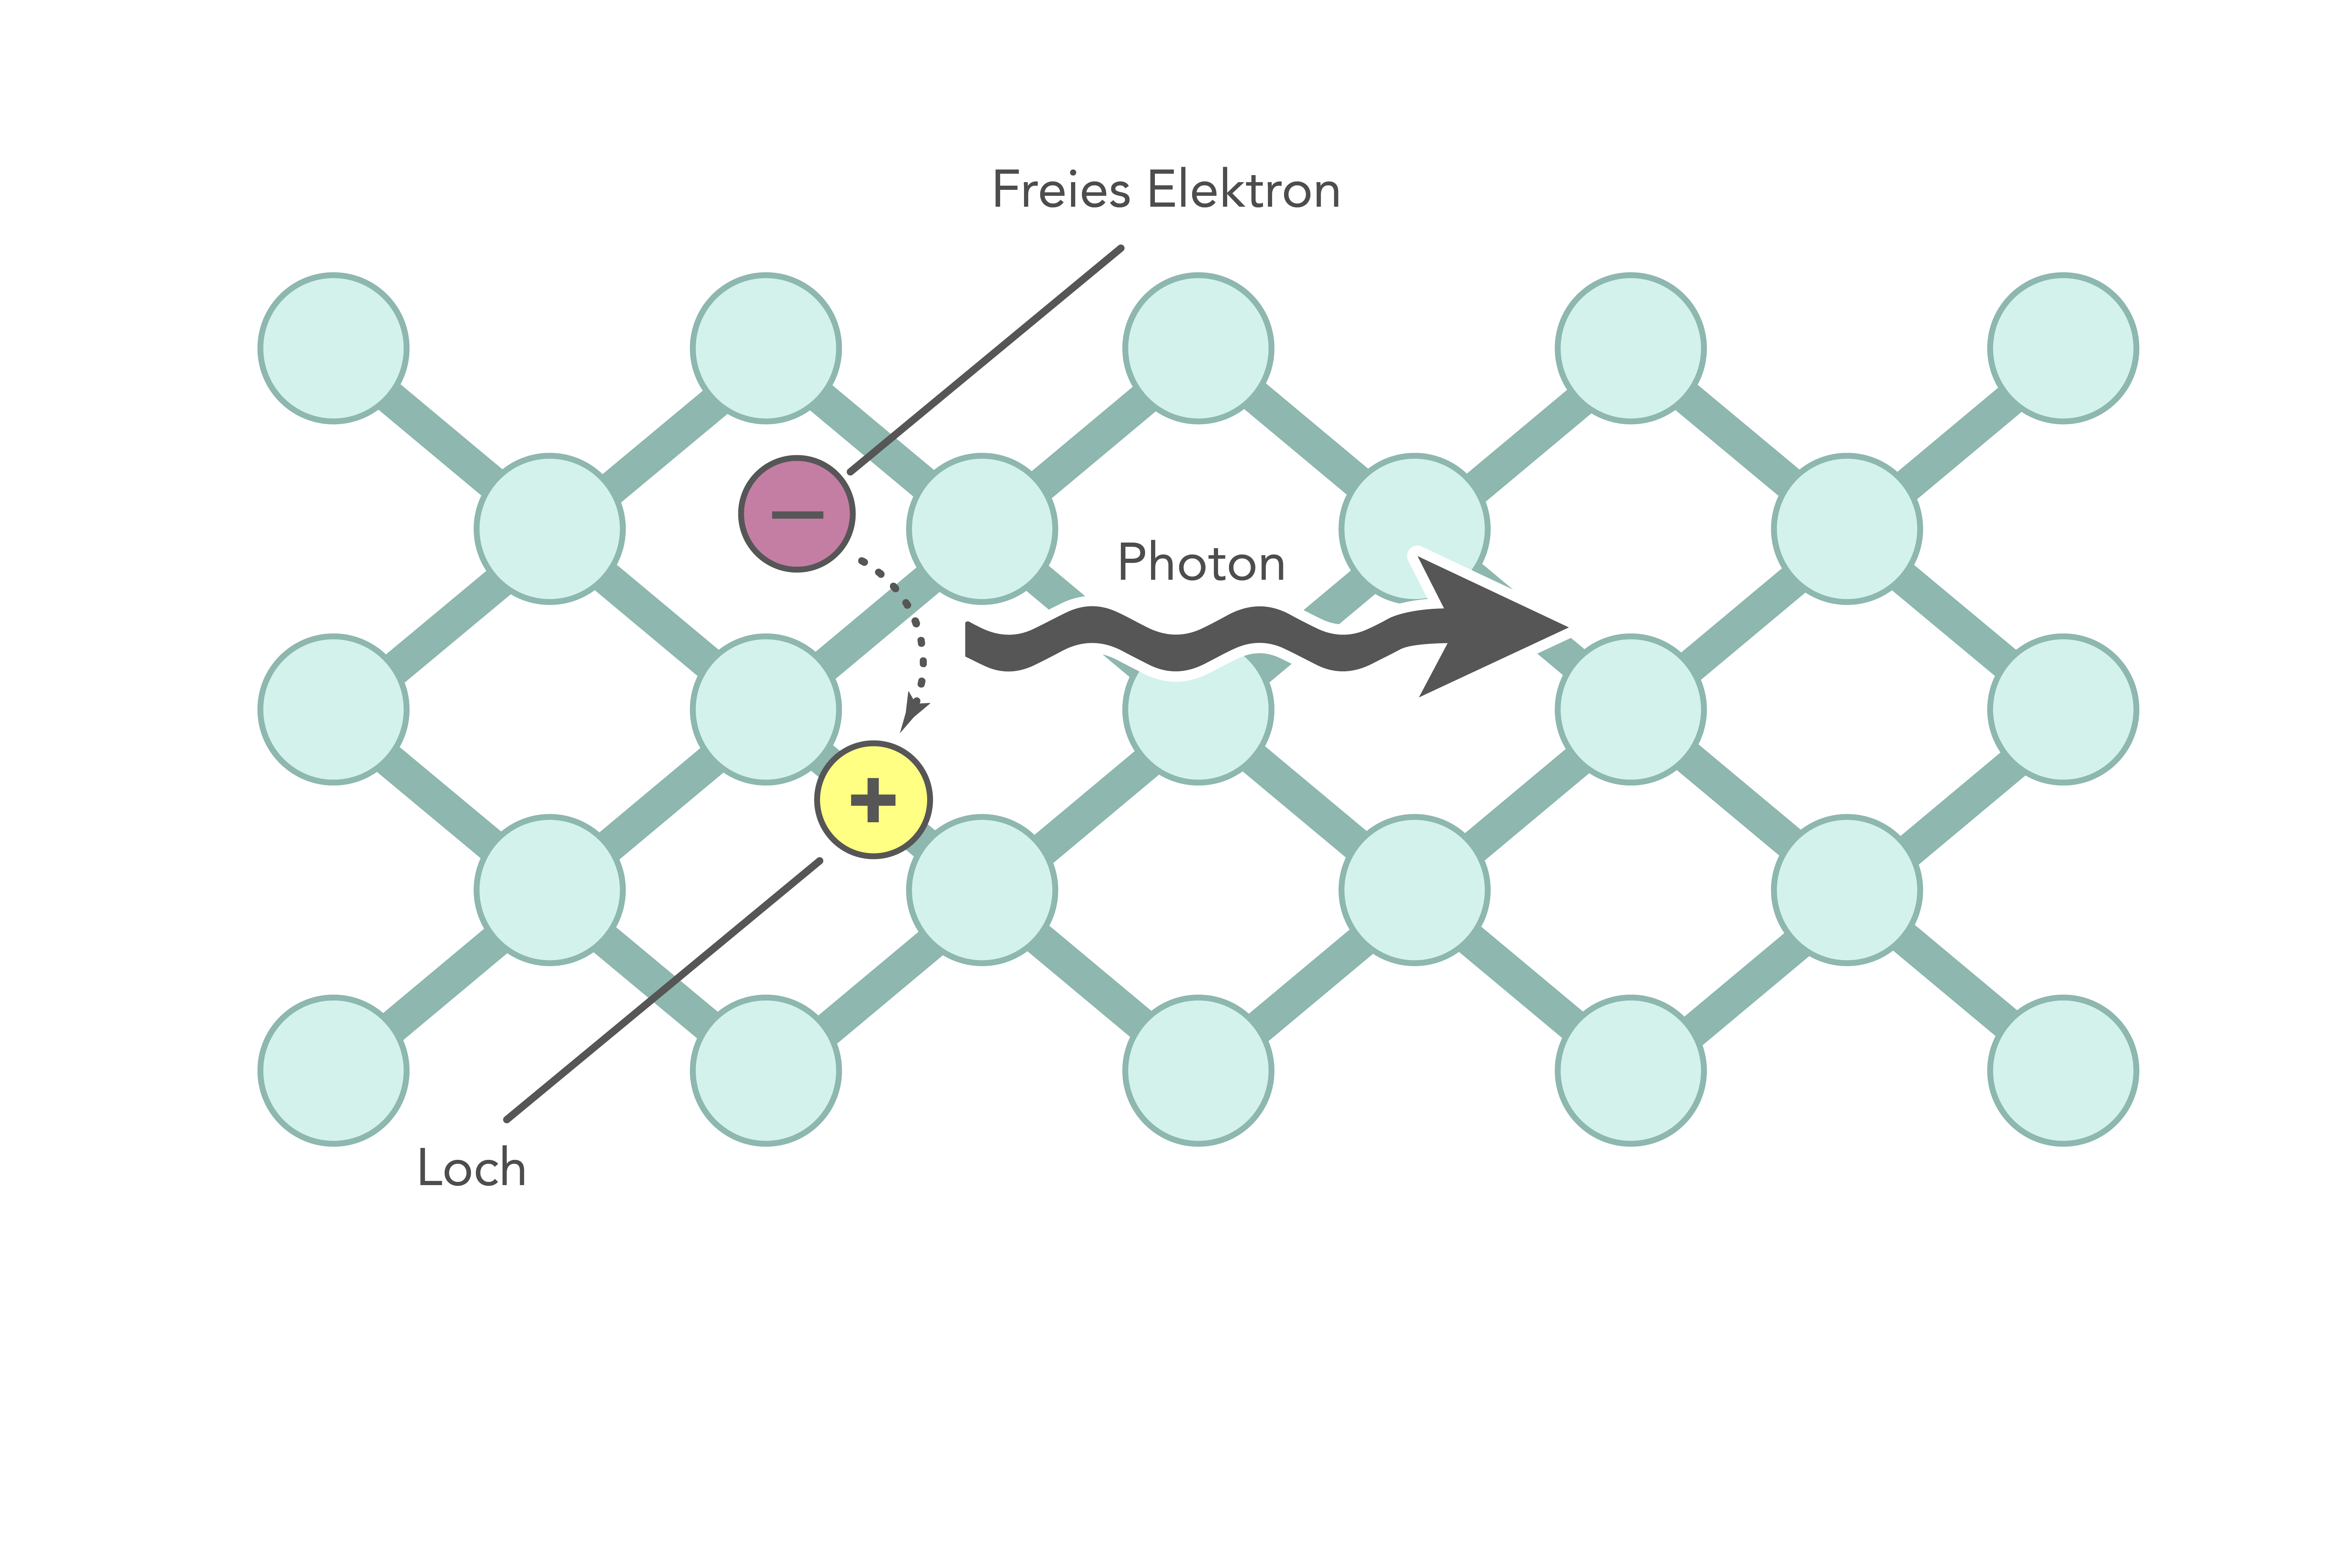
\includegraphics[width=\linewidth]{Bilder/radRekomb.png}
        \caption{Radiative Rekombination von Elektron und Loch und Aussendung eines Photons}
    \end{minipage}
\end{figure}
\raggedright
%
In der Photolumineszenzspektroskopie wird Licht als Anregungsquelle für die Anregung von Halbleitermaterialien für die Erzeugung eines Elektron-Loch-Paars benutzt. Dabe wird ein Elektron aus dem Valenzband in das Leitungsband angehoben und ein Loch zurückgelassen. Die Elektronen relaxieren anschliessend sehr schnell in das Minimum des Leitungsbandes und analog die Löcher in das Minimum des Valenzbandes Abb. . Leitung-und Valenzband befinden sich im Fall von AlGaN am gleichen $\vec{k}$ Vektor im reziproken Raum, dem sog. $\Gamma$ -Punkt. Das macht das Materialsystem AlGaN zu einem direkten Halbleiter, was von besonderem Vorteil ist. Denn ein direkter Bandübergang, ist die wichtigste Grundlage für eine effiziente halbleiterbasierte Lichtquelle. Denn die Wahrscheinlichkeit einer Anregung und daraufhin folgender Rekombination unter Aussendung eines Photons ist deutlich höher, da kein Phonon am Prozess beteiligt sein muss. 
Die Rekombination kann dennoch auch nicht-strahlend erfolgen, weil epitaktisch gewachsene Halbleitersstrukturen herstellungsbedingt beispielsweise nicht ohne ungewollte Dotierung durch Fremdatome, Versetzungen oder Fehlstellen an Atomgitterplätzen (Vakanzen) gewachsen werden können. Diese als sogenannten Störstellen fungieren und diskrete Energieniveaus haben, 
%
\begin{figure}[h]
    \centering
    \begin{minipage}[t]{0.75\linewidth}
        \centering
        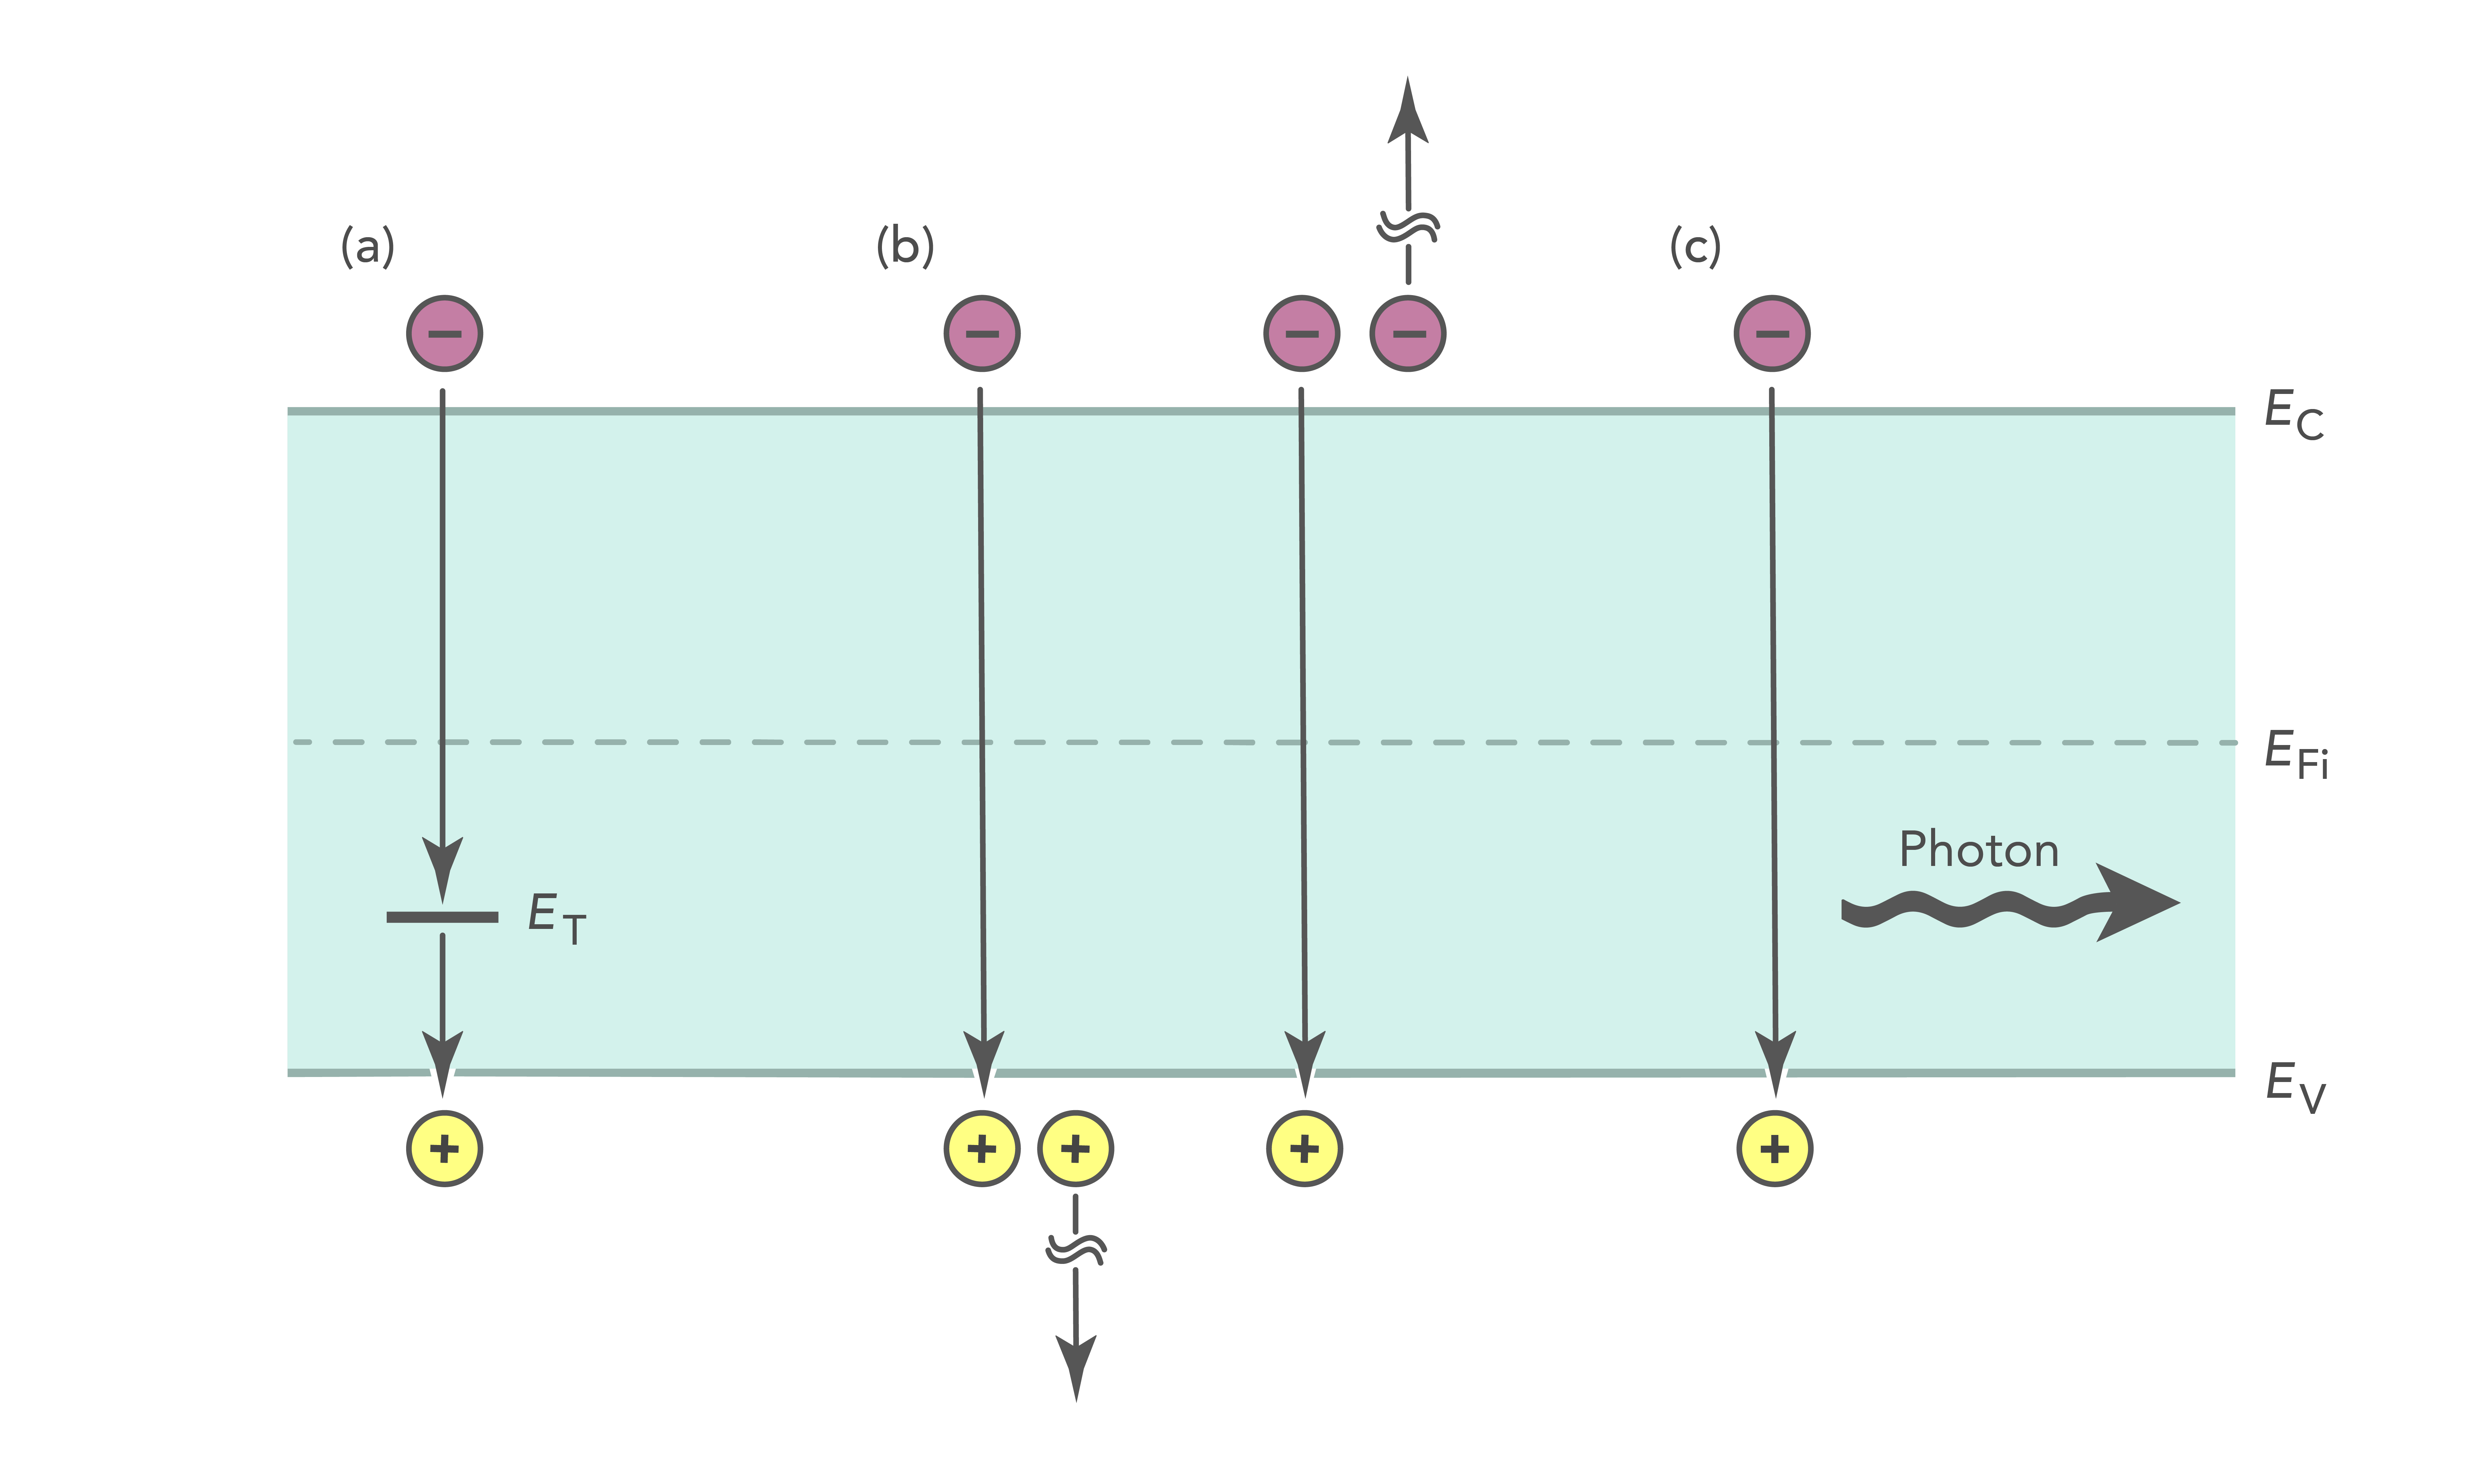
\includegraphics[width=\linewidth]{Bilder/rekbomChannels.png}
        \caption{}
        \label{fig:rekombChannels}
    \end{minipage}% <- sonst wird hier ein Leerzeichen eingefügt
\end{figure}
\raggedright
%
Dazu werden drei Prozesse betrachtet: Zuallerst die nichtstrahlende Rekombination, die durch die Shockley-Read-Hall- (SRH-) Rekombination an Defekten beschrieben und durch den Parameter $A$ berücksichtigt wird ($R_{nonrad} = A \cdot nicht $). Sie ist linear abhängig von der Ladungsträgerdichte $n$. Sie findet statt unter der Beteiligung eines Defektniveaus und eines Phonons. Der strahlende Prozess der spontanen Rekombination ist für niedrige Ladungsträgerdichten quadratisch in $n$ und findet statt als Zwei-Teilchen Prozess bei dem Loch und Elektron beteiligt sind ($R_{rad} = B \cdot n^2 $). Dieser wird beschrieben mit dem Koeffizienten B. 
Der letzte Prozess ist die Auger-Rekombination der speziell für sehr hohe Anregungsleistungsdichten relevant ist und dann durch die kubische Abhängigkeit stark dominiert ($R_{auger} = C \cdot n^3 $). Dabei gibt ein bereits in das Leitungsband angeregte Elektron seine Energie an ein weiteres Elektron im Leitungsband ab. Dieses relaxiert dann entweder wieder zum Leitungsbandminimum unter Mitwirkung von Phononen oder verlässt bei Oberflächennähe den Kristall. Der letzte Fall bildet die Grundlage für die Auger-Elektronen-Spektroskopie.
Die effektive Rekombination ist somit die Summe aus der radiativen Rekombination, der nicht-radiativen Rekombination und der Auger-Rekombination.
\begin{equation}
    R_{eff} = R_{rad} + R_{nonrad} + R_{auger}
    \label{eq:iqe1}
\end{equation}
Der allgemein verwendete Ansatz zur Beschreibung der effektiven Rekombinationsrate $R_{eff}$ (oder auch Generationsrate $G$) wird mit Hilfe der genannten Koeffizienten beschrieben und beruht auf der Abhängigkeit der beteiligten Prozesse von der Ladungsträgerdichte $n$ und wird daher auch ABC-Modell genannt.
\begin{equation}
    R_{eff} (G) = A \cdot n + B \cdot n^2 + C \cdot n^3 
    \label{eq:iqe2}
\end{equation}
Weiter wird angenommen, dass die Anregungsleistungsdichte des Lasers P proportional zu
der Ladungsträger-Generationsrate G ist. Die radiative Rekombination $R_{rad}$ wird hauptsächlich beeinflusst durch den Überlapp der Wellenfunktionen von Elektronen und Loch im Leitungsband und Valenzband des QW. Dieser wiederum ist stark beeinflusst vom QCSE (Abb. 
[\ref{fig:qcse}] ) und besonders bedeutend bei heteroepitaktisch gewachsenen Halbleiterstrukturen. 
%
